\documentclass[a4paper,norsk, 10pt]{article}
\usepackage[utf8]{inputenc}
\usepackage{verbatim}
\usepackage{listings}
\usepackage{graphicx}
\usepackage[norsk]{babel}
\usepackage{a4wide}
\usepackage{color}
\usepackage{amsmath}
\usepackage{float}
\usepackage{amssymb}
\usepackage[dvips]{epsfig}
\usepackage[toc,page]{appendix}
\usepackage[T1]{fontenc}
\usepackage{cite} % [2,3,4] --> [2--4]
\usepackage{shadow}
\usepackage{hyperref}
\usepackage{titling}
\usepackage{marvosym }
\usepackage{subcaption}
\usepackage[noabbrev]{cleveref}
\usepackage{cite}


\setlength{\droptitle}{-10em}   % This is your set screw

\setcounter{tocdepth}{2}

\lstset{language=c++}
\lstset{alsolanguage=[90]Fortran}
\lstset{alsolanguage=Python}
\lstset{basicstyle=\small}
\lstset{backgroundcolor=\color{white}}
\lstset{frame=single}
\lstset{stringstyle=\ttfamily}
\lstset{keywordstyle=\color{red}\bfseries}
\lstset{commentstyle=\itshape\color{blue}}
\lstset{showspaces=false}
\lstset{showstringspaces=false}
\lstset{showtabs=false}
\lstset{breaklines}
\title{AST4320 Oblig 2}
\author{Daniel Heinesen, daniehei}
\begin{document}
\maketitle
\section{Exercise 1}
We have the 1D window function
\begin{equation}
W(x) =
\left\{
	\begin{array}{ll}
		1  & \mbox{if } |x| < R \\
		0 & \mbox{else } 
	\end{array}
\right.
\end{equation}
We now want to find the Fourier transform of this function. We do this straight forward from the definition of the Fourier transform
\begin{equation}
\tilde{W}(k) = \int_{-\infty}^{\infty} W(x) e^{-ikx}dx.
\end{equation}
Inserting our definition of $W(x)$ we find
\begin{equation}
\tilde{W}(k) = \int_{-\infty}^{-R}0\cdot e^{-ikx}dx + \int_{-R}^{R}1\cdot e^{-ikx}dx + \int_{R}^{\infty}0\cdot e^{-ikx}dx = \int_{-R}^{R}e^{-ikx}dx
\end{equation}
\begin{equation}
= \frac{i}{k}e^{-ikx}\bigg|_{-R}^{R} = \frac{i}{k}\left(e^{-ikR} - e^{ikR}\right) = \frac{2\sin Rk}{k}.
\end{equation}
Before we plot this function we need to notice that this is a function that we need to be careful with for $k\rightarrow 0$. With the use of L'Hôpitals rule
\begin{equation}\label{eq:at_0}
 \lim_{ k\rightarrow 0} \tilde{W}(k) = \lim_{k\rightarrow 0} \frac{2 \sin Rk}{k}
= \lim_{k\rightarrow 0} \frac{2R\cos Rk}{1} = 2R. 
 \end{equation}
We now see that $\tilde{W}(k)$ is well defined across the whole real line.

\begin{figure}[H]
\centering
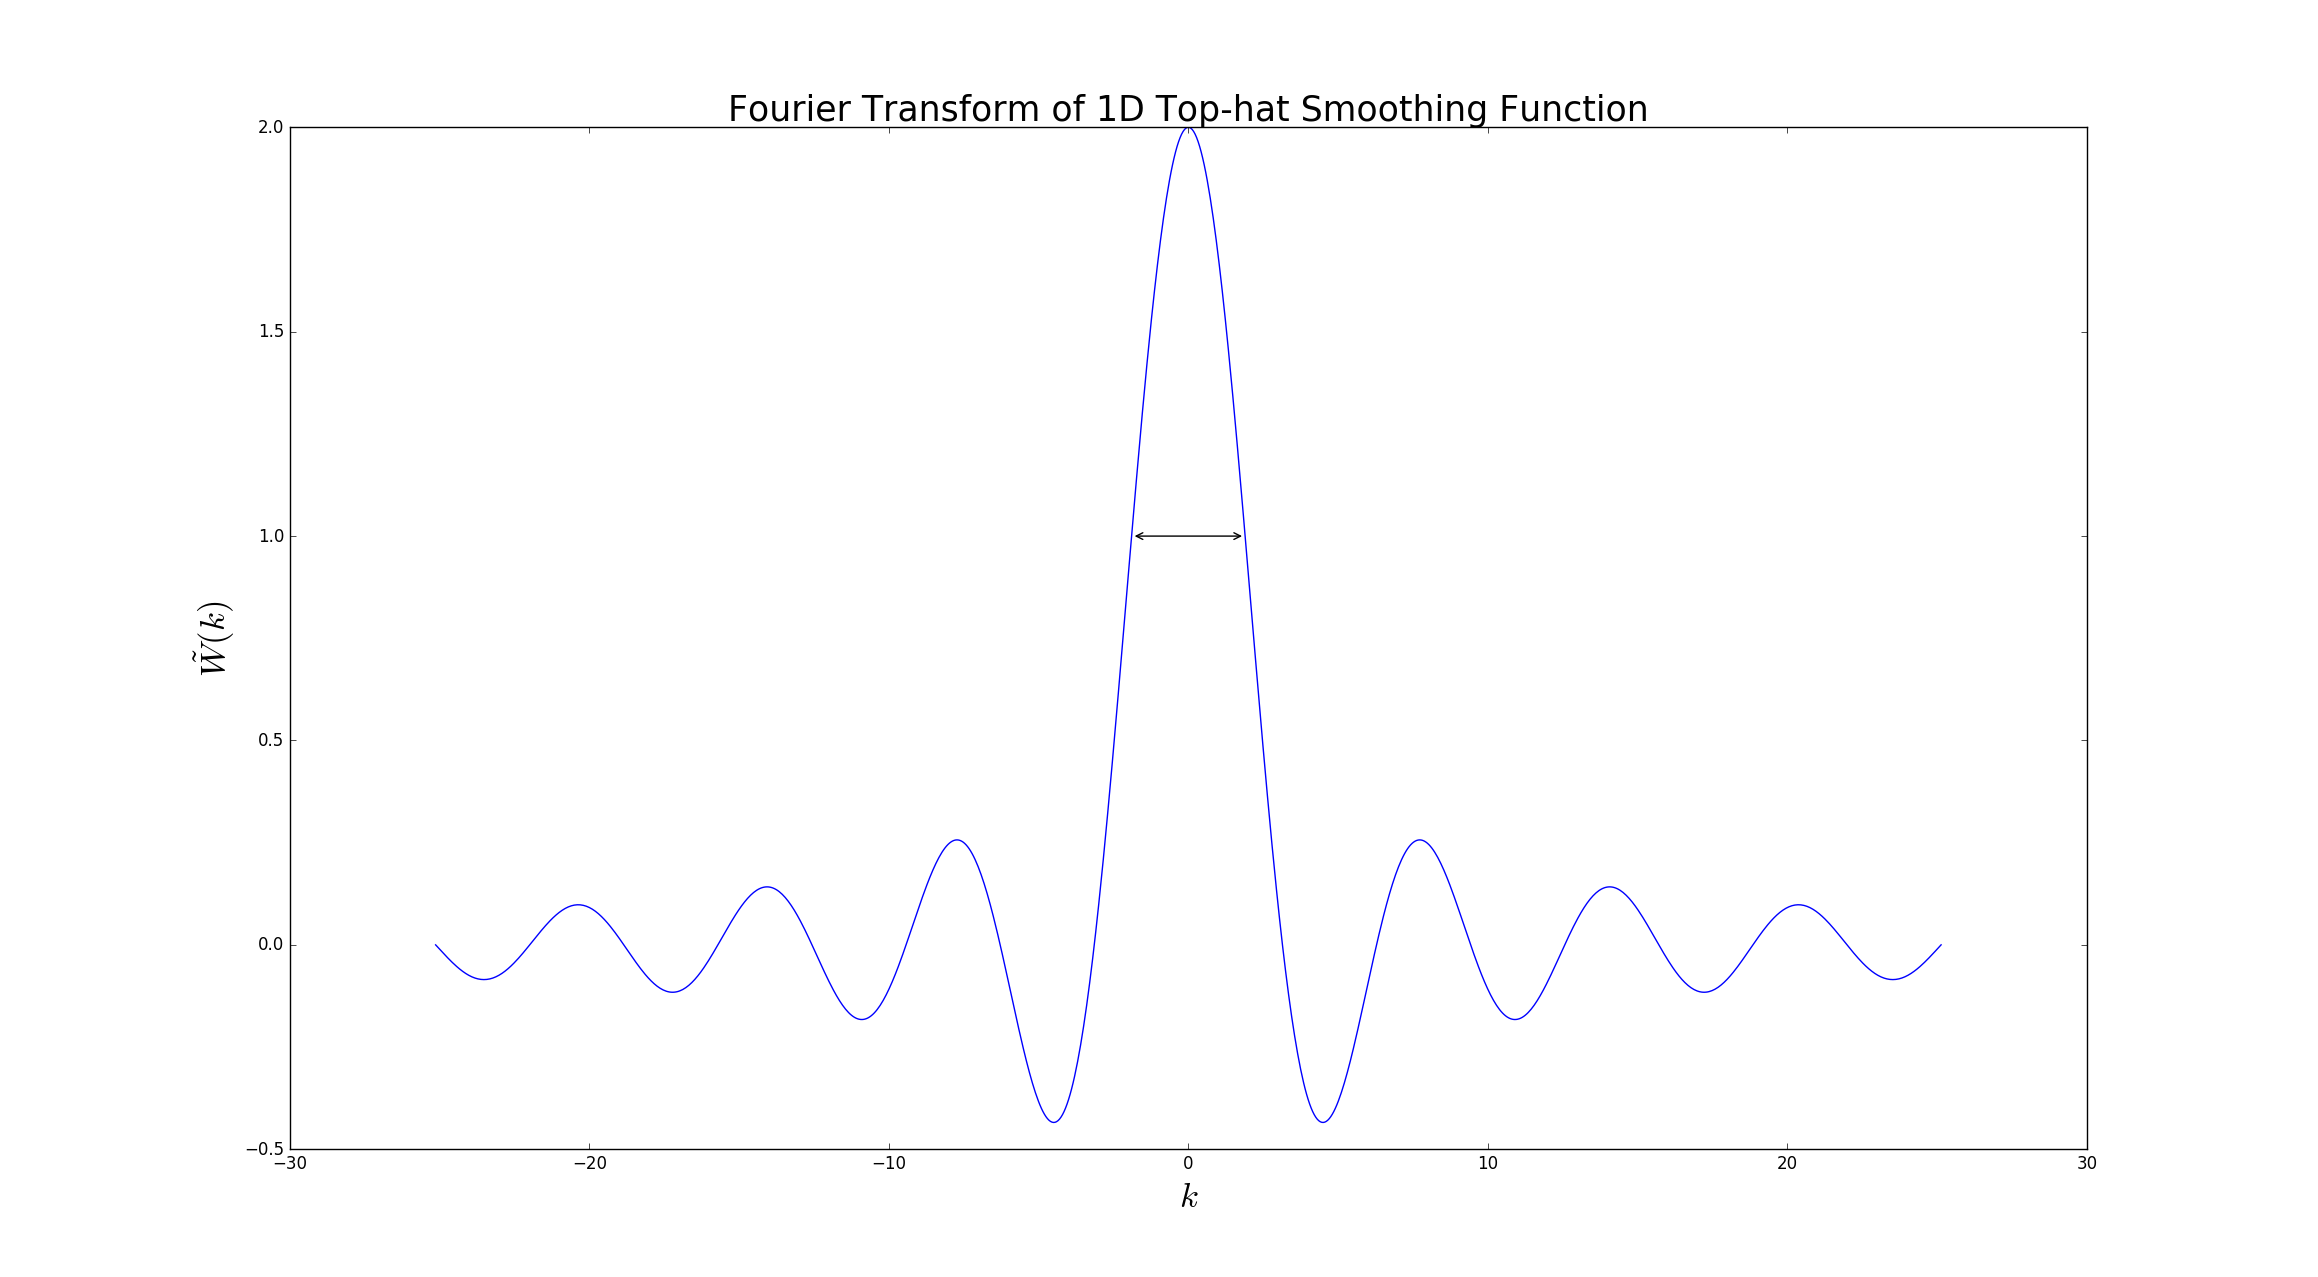
\includegraphics[scale=0.3]{fourier}
\caption{The plot of the Fourier Transform of the top-hat smoothing function $W(x)$. This is plotted with $R=1$. The FWHM is marked with the arrow.}\label{fig:fourier}
\end{figure}

We now want to find the \textit{full width at half maximum}, FWHM, for this function. We first need to find the half maximum. From fig.\ref{fig:fourier} we see that maximum is at $0$. We know from \eqref{eq:at_0} that here $\tilde{W}(k=0) = 2R$, so half maximum is $R$. For the width we just need to find for which $k$ we have $\tilde{W} = R$ and multiply it by $2$ (this is because $\tilde{W}$ is symmetric around $0$). So we first need to solve
\begin{equation}
R = \frac{2}{k_{\text{half max}}}\sin Rk_{\text{half max}}.
\end{equation}
This is difficult to solve analytical, but easy numerically. From our program we easily find that 
\begin{equation}
\text{FWHM} = 2\cdot k_{\text{half max}} = 3.77.
\end{equation}

\section{Exercise 2}

By doing the random walk, found in \textit{ex2.py}, we get the distribution for $\delta$ found in fig. \ref{fig:walk}. We can see that this follows the Gaussian function $\delta \sim N(0,\sigma(M))$. If we restrict our self to the walks that never cross the critical density $\delta_c$ we get the distribution for $\delta_{nc}$ seen in fig. \ref{fig:restricted_walk}. To make the hight of the analytical distribution fit that of the simulated data, I had to multiply it with a fudge factor of $2.2$. Even with this fudge factor the simulated distribution is skewed to the right, with a dramatic cut off point at $\delta = 1$. This cut off point is expected since we restrict out walks to $\delta < \delta_c = 1$, but the cut off is a bit sharp. With a lower $\epsilon$ this becomes smaller, but the code takes to long to run.

\begin{figure}[H]
\centering
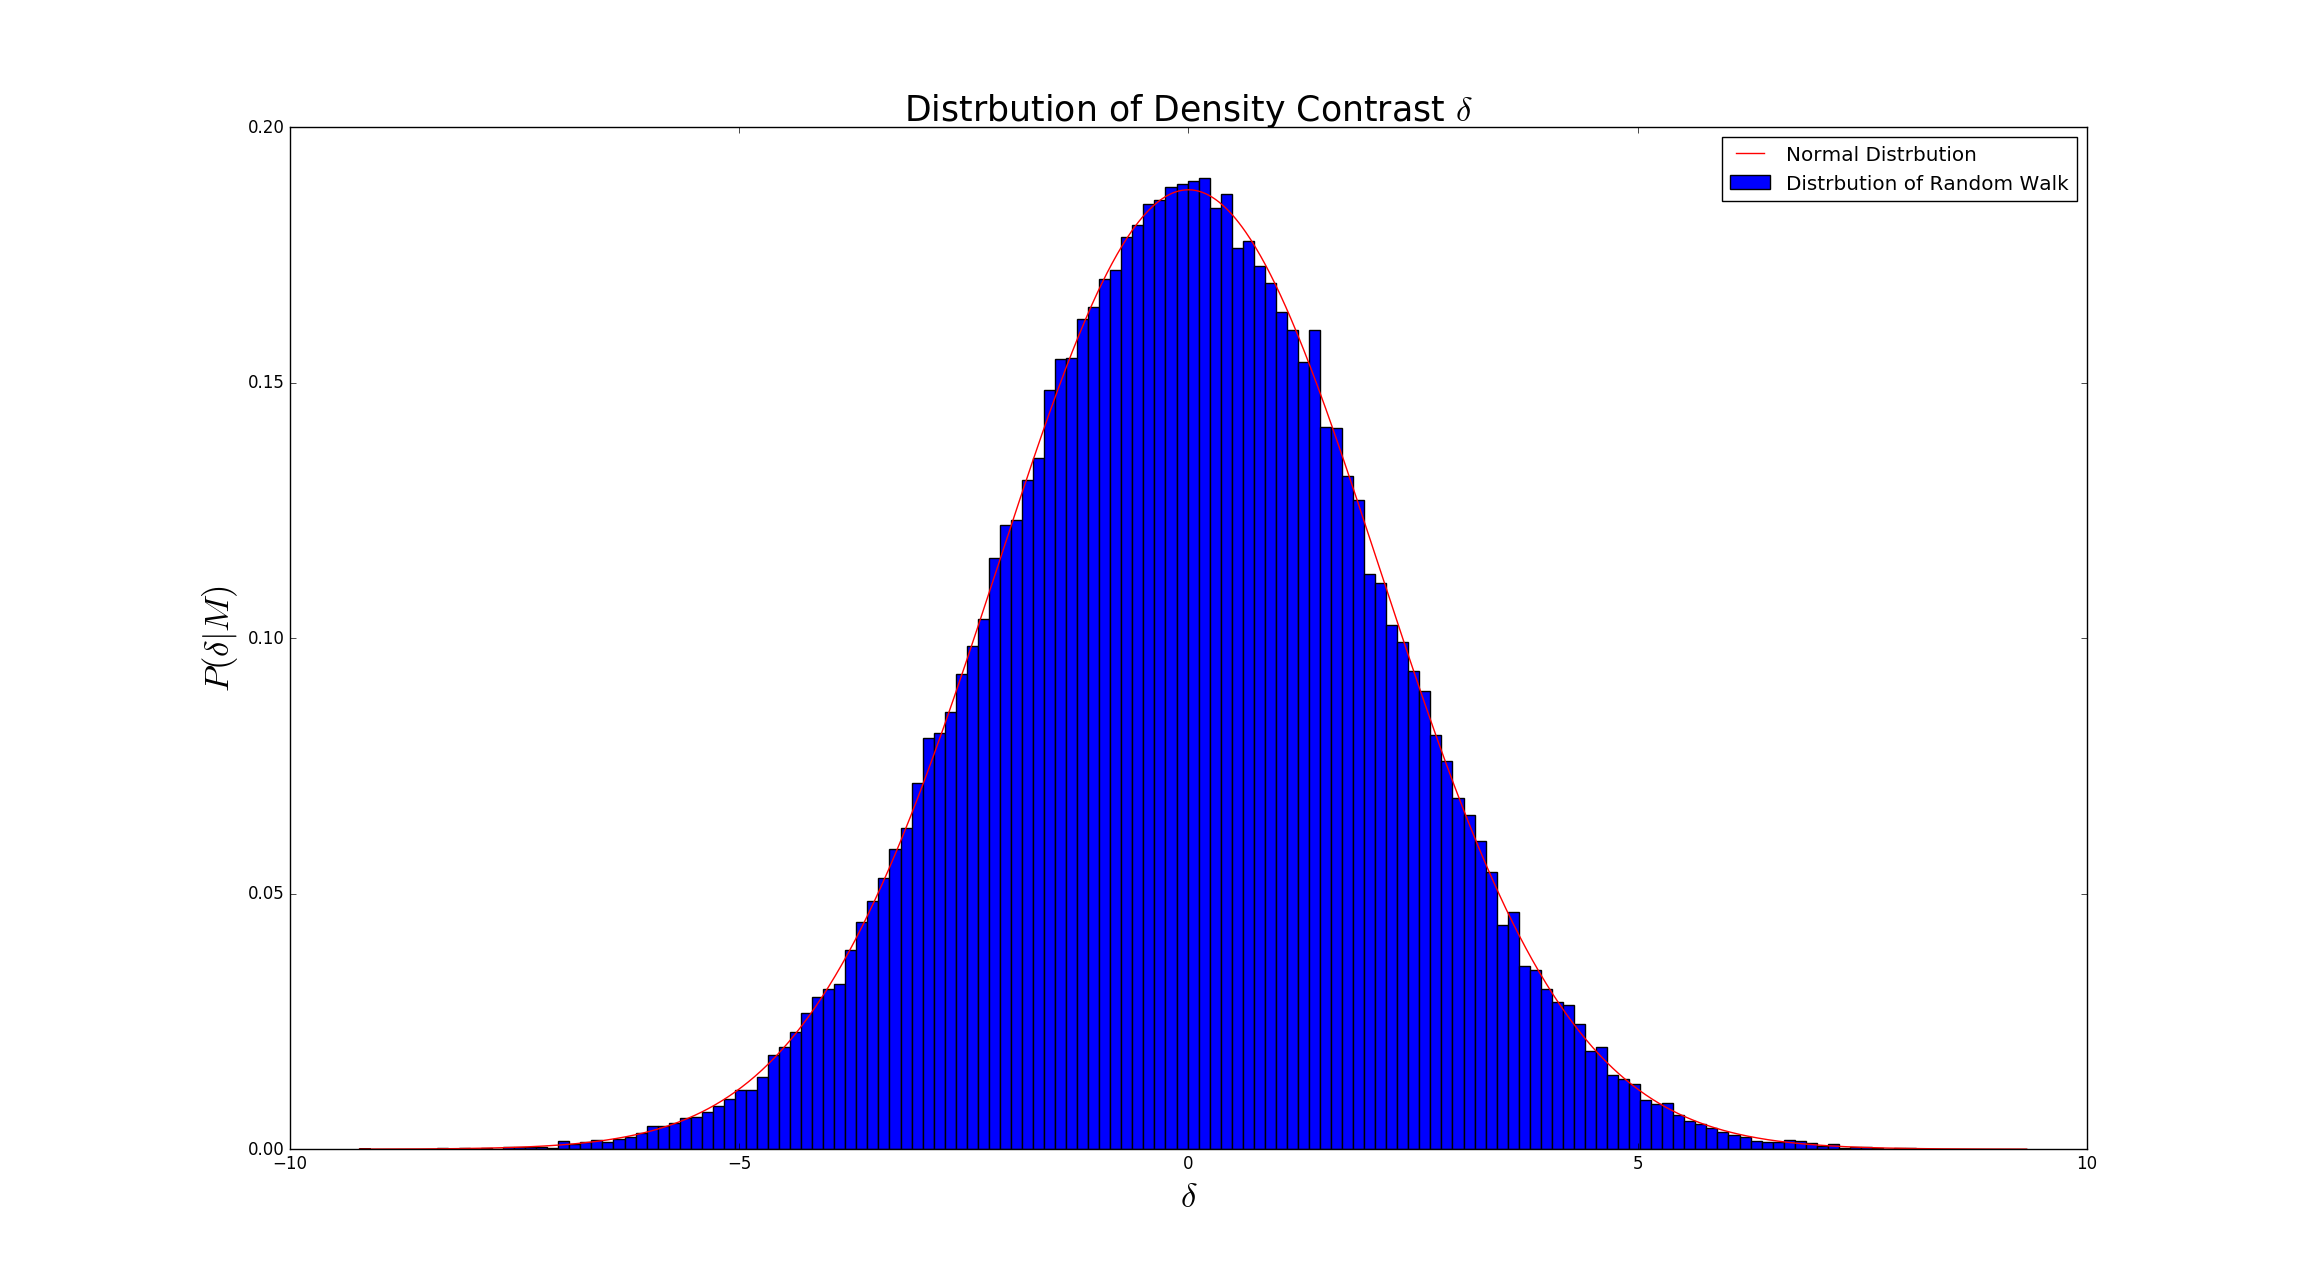
\includegraphics[scale=0.3]{dist}
\caption{Distribution of the endstep in the random walk, simulated with $\epsilon = 0.1$ and $10^5$ walks. We see that this follows a Gaussian distribution with $\sigma^2 = \pi$.}\label{fig:walk}
\end{figure}

\begin{figure}[H]
\centering
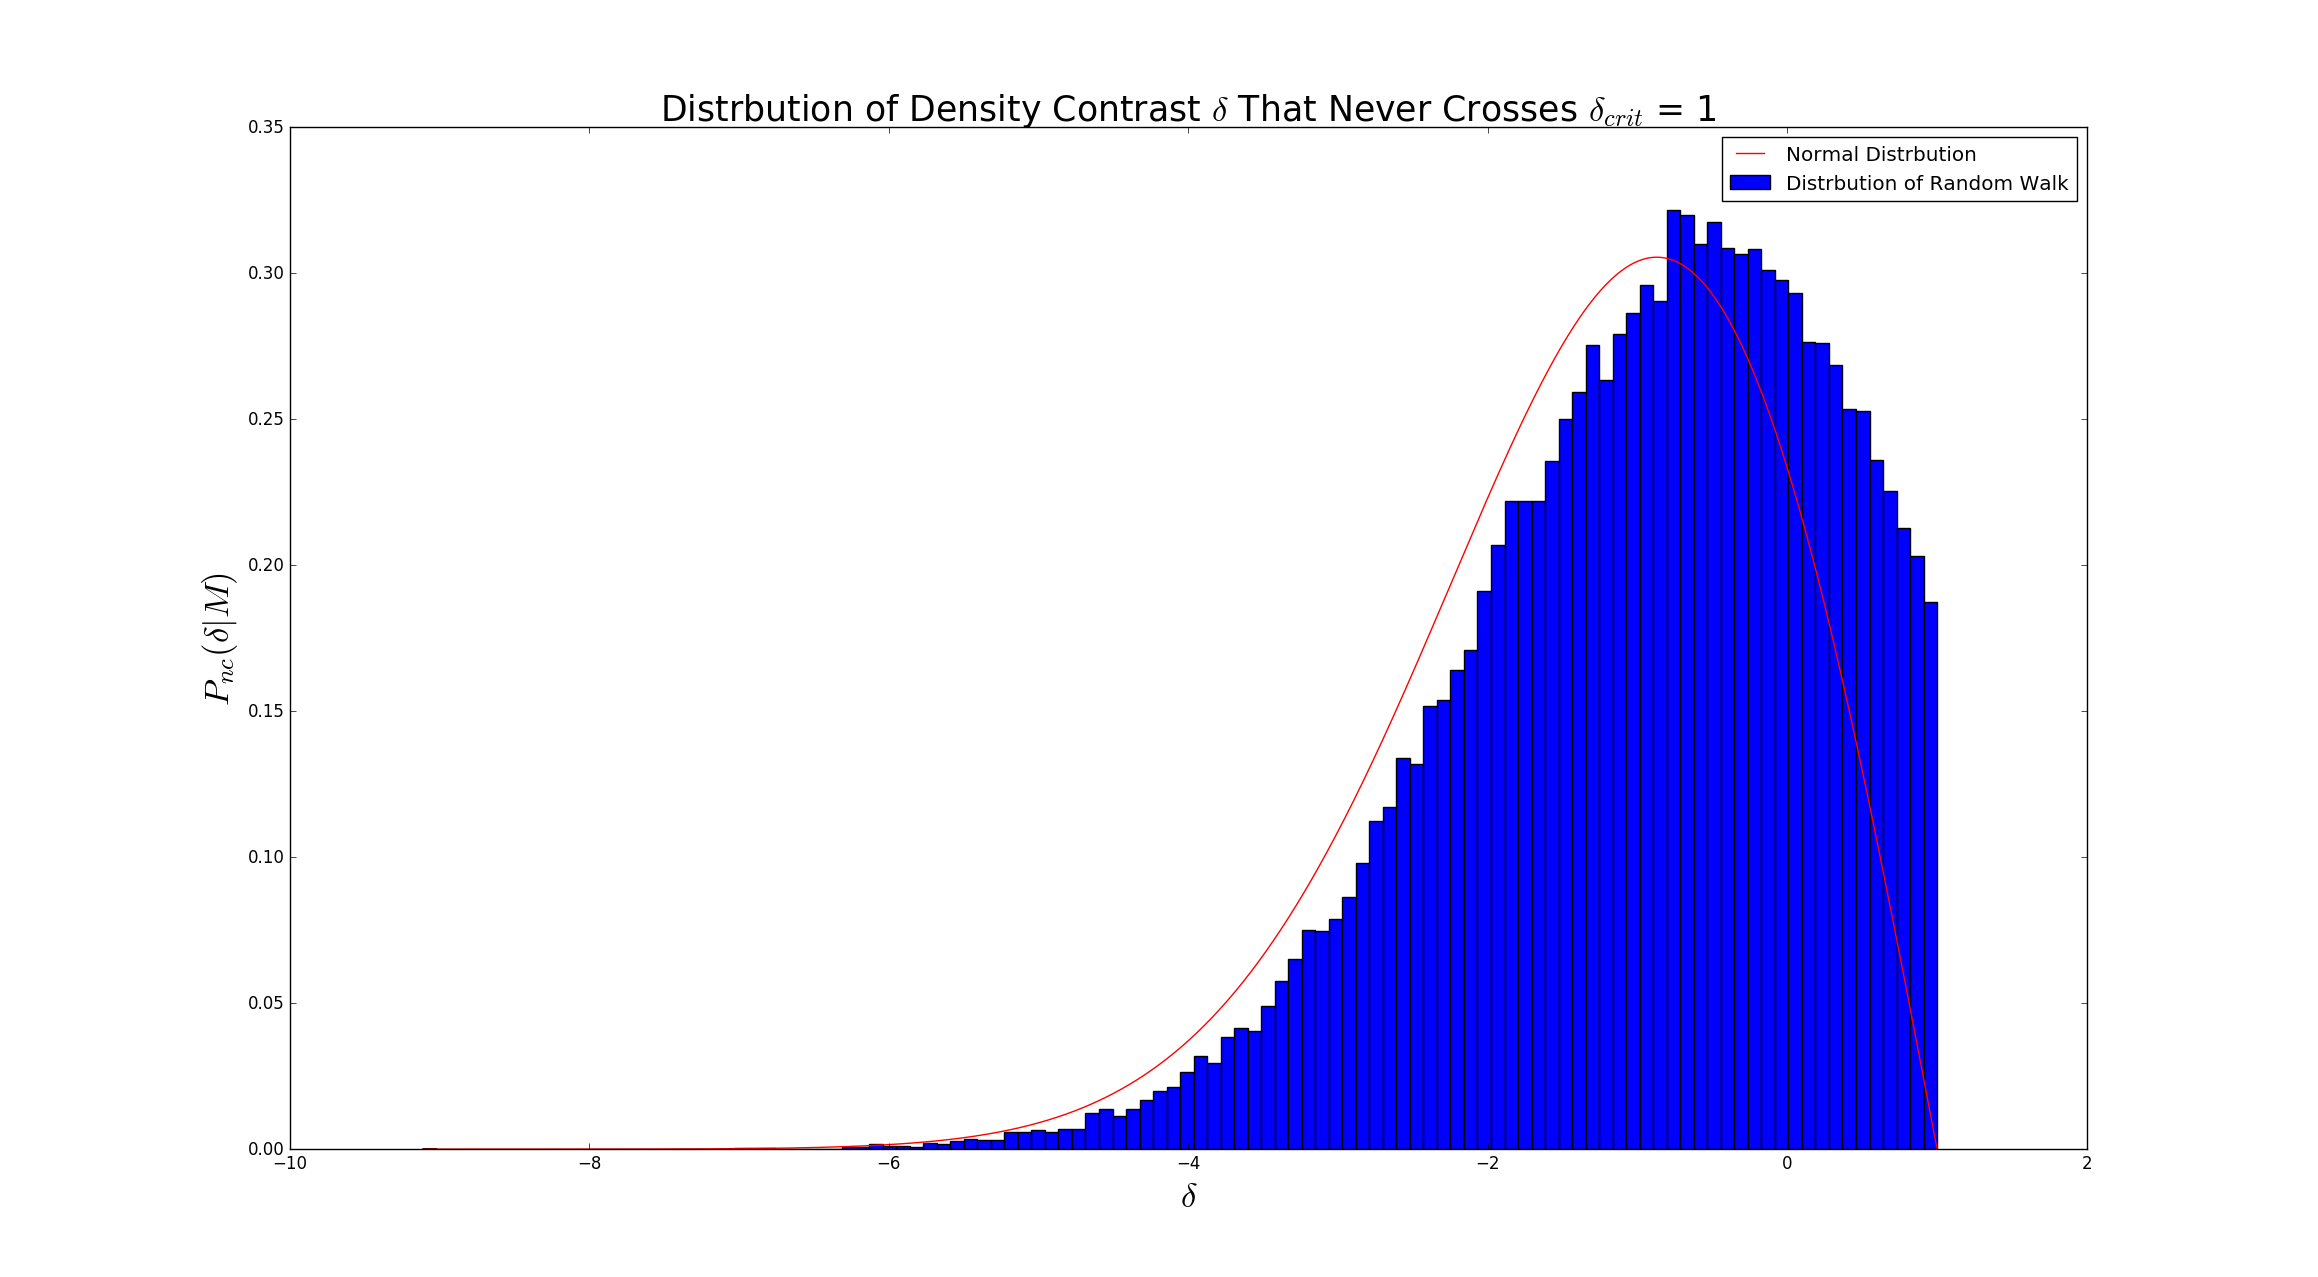
\includegraphics[scale=0.3]{dist_under_crit}
\caption{Distribution of the endstep in the random walk, simulated with $\epsilon = 0.1$ and $10^5$ walks. We can see that distribution is a bit of the expected distribution, even with a $2.2$ fudge factor.}\label{fig:restricted_walk}
\end{figure}


\section{Exercise 3}

\subsection{a)}
We have that the probability of $\delta$ provided that $\delta$ was never larger than $\delta_{crit}$ at some scale $M' > M$ is
\begin{equation}\label{eq:Pnc}
P_{nc}(\delta|M) = \frac{1}{\sqrt{2\pi}\sigma(M)}\left[\exp\left(-\frac{\delta^2}{2\sigma^2 (M)}\right)-\exp\left(-\frac{(2\delta_{crit} - \delta)^2}{2\sigma^2 (M)}\right)\right].
\end{equation}
Since $\delta$ never has crossed $\delta_{crit}$ it is safe to assume that collapse has never happened here. This means that the probability of a mass at $\mathbf{x}$ is  therefore  embedded  within  a  \textit{non}-collapsed object of mass $>M$ is therefore
\begin{equation}
\int_{-\infty}^{\delta_{crit}} P_{nc}(\delta|M) d\delta.
\end{equation}
This means that the probability that this mass is within a collapsed mass is 1 minus this probability. So
\begin{equation}\label{eq:Pm}
P(>M) = 1 - \int_{-\infty}^{\delta_{crit}} P_{nc}(\delta|M) d\delta.
\end{equation}

\subsection{b)}
Using \eqref{eq:Pm} and \eqref{eq:Pnc} we get

\begin{equation}\label{eq:Pm}
P(>M) = 1 - \int_{-\infty}^{\delta_{crit}} \frac{1}{\sqrt{2\pi}\sigma(M)}\left[\exp\left(-\frac{\delta^2}{2\sigma^2 (M)}\right)-\exp\left(-\frac{(2\delta_{crit} - \delta)^2}{2\sigma^2 (M)}\right)\right] d\delta
\end{equation}
\begin{equation}
= 1 - \underbrace{\int_{-\infty}^{\delta_{crit}} \frac{1}{\sqrt{2\pi}\sigma(M)}\left[\exp\left(-\frac{\delta^2}{2\sigma^2 (M)}\right)\right]d\delta}_{I_1}+\underbrace{\int_{-\infty}^{\delta_{crit}} \frac{1}{\sqrt{2\pi}\sigma(M)}\left[\exp\left(-\frac{(2\delta_{crit} - \delta)^2}{2\sigma^2 (M)}\right)\right] d\delta}_{I_2}.
\end{equation}
We then look at this term by term:
\subsubsection*{$I_1$:}
We know that we want something with an error function. To get this we see that we need to introduce the variable
\begin{equation}
u = \frac{\delta}{\sqrt{2}\sigma},
\end{equation}
which gives
\begin{equation}
\Rightarrow \frac{du}{d\delta} = \frac{1}{\sqrt{2}\sigma} \Rightarrow d\delta = \sqrt{2}\sigma du.
\end{equation}
We need to take care of the upper limit $u_{\uparrow}$. We see that this becomes
\begin{equation}
\delta_{\uparrow} = \delta_{crit} = \sqrt{2}\sigma u_{\uparrow} \Rightarrow u_{\uparrow} = \frac{\delta_{crit}}{\sqrt{2}\sigma} \equiv \frac{\nu}{\sqrt{2}}.
\end{equation}
We can then solve $I_1$ as
\begin{equation}
I_1 = \frac{1}{2}\int_{-\infty}^{\nu/\sqrt{2}} \frac{2}{\sqrt{\pi}}e^{-u^2} du.
\end{equation}
Looking this up on integration tables we find that this is
\begin{equation}
I_1 = \frac{1}{2}\left[1+\text{erf}\left(\frac{\nu}{\sqrt{2}}\right)\right]
\end{equation}
\subsubsection*{$I_2$:}
This integral is quite similar to $I_1$, so we use a similar variable change
\begin{equation}
u = \frac{2\delta_{crit}-\delta}{\sqrt{2}\sigma},
\end{equation}
which gives us
\begin{equation}\label{eq:du}
\Rightarrow \frac{du}{d\delta} = -\frac{1}{\sqrt{2}\sigma} \Rightarrow d\delta = -\sqrt{2}\sigma du.
\end{equation}
We now need to look at the limits. While the upper limit stays the same, we need to take a look at the lower limit
\begin{equation}
\delta_{\downarrow} = x = 2\delta_{crit} - \sqrt{2}u_{\downarrow}\sigma \Rightarrow = u_{\downarrow} = \frac{2\delta_{crit} - x}{\sqrt{2}\sigma}, 
\end{equation}
then taking the limit of $x$ we get
\begin{equation}
u_{\downarrow} =\lim_{x \rightarrow -\infty} \frac{2\delta_{crit} - x}{\sqrt{2}\sigma} = \infty.
\end{equation}
We can then use the minus sign from \eqref{eq:du} to turn the limits around and get
\begin{equation}
I_2 = \frac{1}{2}\int_{\nu/\sqrt{2}}^{\infty}\frac{2}{\sqrt{\pi}}e^{-u^2} du = \frac{1}{2}\text{erfc}\left(\frac{\nu}{\sqrt{2}}\right) = \frac{1}{2}\left[1-\text{erf}\left(\frac{\nu}{\sqrt{2}}\right)\right]
\end{equation}

We thus get the probability
\begin{equation}
P(>M) = 1-I_1 + I_2 = 1 - \frac{1}{2}\left[1+\text{erf}\left(\frac{\nu}{\sqrt{2}}\right)\right] + \frac{1}{2}\left[1-\text{erf}\left(\frac{\nu}{\sqrt{2}}\right)\right] = 1 - \text{erf}\left(\frac{\nu}{\sqrt{2}}\right) = 2P(\delta > \delta_{crit}|M).
\end{equation}
And there is no need for the fudge factor!



\end{document}

